\documentclass[12pt,letterpaper]{exam}
\usepackage[lmargin=1in,rmargin=1in,tmargin=1in,bmargin=1in]{geometry}
\usepackage{../style/exams}

% -------------------
% Course & Exam Information
% -------------------
\newcommand{\course}{MAT 108: Exam 3}
\renewcommand{\term}{Spring -- 2023}
\newcommand{\examdate}{05/03/2023}
\newcommand{\timelimit}{85 Minutes}

\setbool{hideans}{false} % Student: True; Instructor: False

% -------------------
% Content
% -------------------
\begin{document}

\examtitle
\instructions{Write your name on the appropriate line on the exam cover sheet. This exam contains \numpages\ pages (including this cover page) and \numquestions\ questions. Check that you have every page of the exam. Answer the questions in the spaces provided on the question sheets. Be sure to answer every part of each question and show all your work. If you run out of room for an answer, continue on the back of the page --- being sure to indicate the problem number.} 
\scores
\bottomline
\newpage

% ---------
% Questions
% ---------
\begin{questions}

% Question 1
\newpage
\question[10] Define the following vectors:
	\[
	\mathbf{u}= \begin{pmatrix} 3 \\ -2 \\ 0 \end{pmatrix} \qquad 
	\mathbf{v}= \begin{pmatrix} -4 \\ 1 \\ 5 \end{pmatrix}
	\]
Showing all your work, compute the following:
	\begin{enumerate}[(a)]
	\item $-2 \mathbf{v}$
	\item $\mathbf{v} - 3 \mathbf{u}$
	\item $\mathbf{u} \cdot \mathbf{v}$
	\end{enumerate} \pspace

\sol 
\begin{enumerate}[(a)]
\item 
	\[
	-2 \mathbf{v}= -2 \begin{pmatrix} -4 \\ 1 \\ 5 \end{pmatrix}= \begin{pmatrix} 8 \\ -2 \\ -10 \end{pmatrix}
	\] \pspace

\item 
	\[
	\mathbf{v} - 3 \mathbf{u}= \begin{pmatrix} -4 \\ 1 \\ 5 \end{pmatrix} - 3 \begin{pmatrix} 3 \\ -2 \\ 0 \end{pmatrix}= \begin{pmatrix} -4 \\ 1 \\ 5 \end{pmatrix} - \begin{pmatrix} 9 \\ -6 \\ 0 \end{pmatrix}= \begin{pmatrix} -4 - 9 \\ 1 - (-6) \\ 5 - 0 \end{pmatrix}= \begin{pmatrix} -13 \\ 7 \\ 5 \end{pmatrix}
	\] \pspace

\item 
	\[
	\mathbf{u} \cdot \mathbf{v}= \begin{pmatrix} 3 \\ -2 \\ 0 \end{pmatrix} \cdot \begin{pmatrix} -4 \\ 1 \\ 5 \end{pmatrix}= 3(-4) + (-2)1 + 0(5)= -12 - 2 + 0= -14
	\]
\end{enumerate}



% Question 2
\newpage
\question[10] Define the following matrices:
	\[
	A= \begin{pmatrix} 1 & 0 & 3 \\ 2 & -1 & 4 \\ 0 & 6 & -2 \end{pmatrix} \qquad
	B= \begin{pmatrix} 1 & 8 \\ -2 & 0 \\ 0 & 3 \\ 9 & -6 \end{pmatrix} \qquad
	C= \begin{pmatrix} 2 & -7 & -9 \\ 3 & 6 & 5 \\ 8 & -2 & -3 \end{pmatrix}
	\]

\begin{enumerate}[(a)]
\item Compute $B^T$. 
\item Showing all your work, compute $-2C$.
\item Showing all your work, compute $C - A$. 
\item Explain why one cannot form the product $AB$. 
\end{enumerate} \pspace

\sol 
\begin{enumerate}[(a)]
\item 
	\[
	B^T= \begin{pmatrix} 1 & 8 \\ -2 & 0 \\ 0 & 3 \\ 9 & -6 \end{pmatrix}^T= \begin{pmatrix} 1 & -2 & 0 & 9 \\ 8 & 0 & 3 & -6 \end{pmatrix}
	\] \pspace

\item 
	\[
	-2C= -2 \begin{pmatrix} 2 & -7 & -9 \\ 3 & 6 & 5 \\ 8 & -2 & -3 \end{pmatrix}= \begin{pmatrix} -4 & 14 & 18 \\ -6 & -12 & -10 \\ -16 & 4 & 6 \end{pmatrix}
	\] \pspace

\item 
	\[
	\begin{aligned}
	\begin{pmatrix} 2 & -7 & -9 \\ 3 & 6 & 5 \\ 8 & -2 & -3 \end{pmatrix} - \begin{pmatrix} 1 & 0 & 3 \\ 2 & -1 & 4 \\ 0 & 6 & -2 \end{pmatrix}&= \begin{pmatrix} 2 - 1 & -7 - 0 & -9 - 3 \\ 3 - 2 & 6 - (-1) & 5 - 4 \\ 8 - 0 & -2 - 6 & -3 - (-2) \end{pmatrix} \\
	&= \begin{pmatrix} 1 & -7 & -12 \\ 1 & 7 & 1 \\ 8 & -8 & -1 \end{pmatrix}
	\end{aligned}
	\] \pspace

\item If $A$ is a $m \times n$ matrix and $B$ is a $r \times s$ matrix, then the product $AB$ can only be formed if $n= r$. If so, the resulting product will have dimension $m \times s$. We know $A$ has dimension $3 \times 3$, i.e. $m= n= 3$, and $B$ has dimension $4 \times 2$, i.e. $r= 4$ and $s= 2$. Because $n= 3 \neq 4= r$, the product $AB$ cannot be formed. 
\end{enumerate}



% Question 3
\newpage
\question[10] Consider the system of linear equations shown below:
	\[
	\begin{aligned}
	2x + 3y&= 1 \\
	4x + 5y&= 5
	\end{aligned}
	\]
Let $A$ be the coefficient matrix and $\mathbf{b}$ be the constant vector associated to the system of equations above. 
        \begin{enumerate}[(a)]
        \item Write the system of equations above in the form $A\mathbf{x}= \mathbf{b}$. 
        \item Explain why $A^{-1}$ exists and find $A^{-1}$. 
        \item Use $A^{-1}$ to find the solution to the system of equations above. 
        \end{enumerate} \par\vspace{0.2cm}

\sol 
\begin{enumerate}[(a)]
\item We choose the order of the variables given by the `alignment' of the variables in the system of equations above. The matrix $A$ is the matrix with columns given by the coefficients of the variables in the selected order. The vector $\mathbf{x}$ is the `variable' vector (in the chosen order). The vector $\mathbf{b}$ is the constant vector. But then we have\dots
	\[
	A= \begin{pmatrix} 2 & 3 \\ 4 & 5 \end{pmatrix} \qquad \mathbf{x}= \begin{pmatrix} x \\ y \end{pmatrix} \qquad \mathbf{b}= \begin{pmatrix} 1 \\ 5 \end{pmatrix}
	\]
But then the given system of equations can be rewritten in the form $A\mathbf{x}= \mathbf{b}$ as\dots
	\[
	 \begin{pmatrix} 2 & 3 \\ 4 & 5 \end{pmatrix} \begin{pmatrix} x \\ y \end{pmatrix}= \begin{pmatrix} 1 \\ 5 \end{pmatrix}
	\] \par\vspace{0.2cm}

\item We know that a square matrix, $M$, has an inverse if and only if $\det M \neq 0$. To check that $A$ has an inverse, we need only check that $\det A \neq 0$. But we have\dots
	\[
	\det A= \det \begin{pmatrix} 2 & 3 \\ 4 & 5 \end{pmatrix}= 2(5) - 3(4)= 10 - 12= -2 \neq 0
	\]
Therefore, $A^{-1}$ exists. However, we know the `form' of the inverse for a two-by-two matrix, $M$, with $\det M \neq 0$. The general form is shown below. We use this to compute $A^{-1}$. 
	\[
	\begin{aligned}
	M&= \begin{pmatrix} a & b \\ c & d \end{pmatrix} \Longrightarrow M^{-1}= \dfrac{1}{\det M} \begin{pmatrix} d & -b \\ -c & a \end{pmatrix} \\[0.3cm]
	A&= \begin{pmatrix} 2 & 3 \\ 4 & 5 \end{pmatrix} \Longrightarrow A^{-1}= \dfrac{1}{-2} \begin{pmatrix} 5 & -3 \\ -4 & 2 \end{pmatrix}
	\end{aligned}
	\] \par\vspace{0.3cm}

\item We know that if we have an equation $A\mathbf{x}= \mathbf{b}$ and $A^{-1}$ exists, we can multiply on the left on both sides of the equation by $A^{-1}$. This yields $A^{-1}A\mathbf{x}= A^{-1}\mathbf{b}$. Because $A^{-1}$ is the inverse of $A$, we know $A^{-1}A= I_2$. But $I_2 \mathbf{x}= \mathbf{x}$. Therefore, we know that $\mathbf{x}= A^{-1} \mathbf{b}$. We simple compute this below. 
	\[
	\hspace{-2.75cm} \begin{pmatrix} x \\ y \end{pmatrix}= \mathbf{x}= A^{-1} \mathbf{b}= \dfrac{1}{-2} \begin{pmatrix} 5 & -3 \\ -4 & 2 \end{pmatrix} \begin{pmatrix} 1 \\ 5 \end{pmatrix}= -\dfrac{1}{2} \begin{pmatrix} 5(1) + (-3)5 \\ -4(1) + 2(5) \end{pmatrix}= -\dfrac{1}{2} \begin{pmatrix} 5 - 15 \\ -4 + 10 \end{pmatrix}= -\dfrac{1}{2} \begin{pmatrix} -10 \\ 6 \end{pmatrix}= \begin{pmatrix} 5 \\ -3 \end{pmatrix}
	\]
Therefore, we know the solution is $(x, y)= (5, -3)$, i.e. $x= 5$ and $y= -3$. 
\end{enumerate}



% Question 4
\newpage
\question[10] The matrix below is the initial augmented matrix coming from a system of linear equations. Find the original system of equations. 
	\[
	\begin{pmatrix} 3 & -1 & 5 & 2 & 8 \\ 7 & 0 & 2 & 8 & -11 \\ 4 & 1 & -1 & 6 & 15 \end{pmatrix}
	\] \pspace

\sol Adding a dashed line to separate matrix entries representing coefficients and those representing constants in the augmented matrix, we have\dots
	\[
	\left(
	\begin{array}{rrrr:r}
	3 & -1 & 5 & 2 & 8 \\ 
	7 & 0 & 2 & 8 & -11 \\ 
	4 & 1 & -1 & 6 & 15
	\end{array} 
	\right)
	\]
There are five columns. The last column corresponds to the constants while the rest correspond to the variables. Therefore, there are four variables. We label our variables $x_1$, $x_2$, $x_3$, and $x_4$. The first four columns represent the coefficients in each equation for the variables $x_1$, $x_2$, $x_3$, and $x_4$, respectively. Then writing out the equation corresponding to each row yields\dots
	\[
	\begin{aligned}
	3x_1 - x_2 + 5x_3 + 2x_4&= 8 \\
	7x_1 + 2x_3 + 8x_4&= -11 \\
	4x_1 + x_2 - x_3 + 6x_4&= 15
	\end{aligned}
	\]



% Question 5
\newpage
\question[10] The matrix shown below is the RREF of an augmented matrix coming from a system of linear equations. Does the corresponding system of equations have a solution? If so, find the solution(s). If not, explain why. 
	\[
	\begin{pmatrix}
	1 & 0 & 0 & 0 & 4 \\
	0 & 1 & 0 & 0 & 0 \\
	0 & 0 & 1 & 0 & -5 \\
	0 & 0 & 0 & 1 & 3
	\end{pmatrix}
	\] \pspace

\sol The original system of equations has a unique solution. Adding a dashed line to separate matrix entries representing coefficients and those representing constants in the RREF augmented matrix, we have\dots
	\[
	\left(
	\begin{array}{rrrr:r}
	1 & 0 & 0 & 0 & 4 \\
	0 & 1 & 0 & 0 & 0 \\
	0 & 0 & 1 & 0 & -5 \\
	0 & 0 & 0 & 1 & 3
	\end{array} 
	\right)
	\]
There are five columns. The last column corresponds to the constants while the rest correspond to the variables. Therefore, there are four variables. We label our variables $x_1$, $x_2$, $x_3$, and $x_4$. The first four columns represent the coefficients in each equation for the variables $x_1$, $x_2$, $x_3$, and $x_4$, respectively. Then writing out the equation corresponding to each row yields\dots
	\[
	\begin{gathered}
	1x_1 + 0x_2 + 0x_3 + 0x_4= 4 \\
	0x_1 + 1x_2 + 0x_3 + 0x_4= 0 \\
	0x_1 + 0x_2 + 1x_3 + 0x_4= -5 \\
	0x_1 + 0x_2 + 0x_3 + 1x_4= 3
	\end{gathered}
	\]
But then we have\dots
	\[
	\begin{gathered}
	x_1= 4 \\
	x_2= 0 \\
	x_3= -5 \\
	x_4= 3
	\end{gathered}
	\]
Therefore, the solution to the original system of equations is $(x_1, x_2, x_3, x_4)= (4, 0, -5, 3)$, i.e.
	\[
	\begin{cases}
	x_1= 4 \\
	x_2= 0 \\
	x_3= -5 \\
	x_4= 3	
	\end{cases}
	\]
 


% Question 6
\newpage
\question[10] The matrix shown below is the REF of an augmented matrix coming from a system of linear equations. Does the corresponding system of equations have a solution? If so, find the solution(s). If not, explain why. 
	\[
	\begin{pmatrix}
	1 & 0 & 0 & -1 \\
	0 & 1 & 0 & 9 \\
	0 & 0 & 1 & 2 \\
	0 & 0 & 0 & 1
	\end{pmatrix}
	\] \pspace

\sol The original system of equations does not have a solution. Adding a dashed line to separate matrix entries representing coefficients and those representing constants in the REF augmented matrix, we have\dots
	\[
	\left(
	\begin{array}{rrrr:r}
	1 & 0 & 0 & -1 \\
	0 & 1 & 0 & 9 \\
	0 & 0 & 1 & 2 \\
	0 & 0 & 0 & 1
	\end{array} 
	\right)
	\]
There are four columns. The last column corresponds to the constants while the rest correspond to the variables. Therefore, there are three variables. We label our variables $x_1$, $x_2$, and $x_3$. Then writing out the equation corresponding to each row yields\dots
	\[
	\begin{gathered}
	x_1 + 0x_2 + 0x_3= -1 \\
	0x_1 + x_2 + 0x_3= 9 \\
	0x_1 + 0x_2 + x_3= 2 \\
	0x_1 + 0x_2 + 0x_3= 1
	\end{gathered}
	\]
But then we have\dots
	\[
	\begin{gathered}
	x_1= -1 \\
	x_2= 9 \\
	x_3= 2 \\
	0= 1
	\end{gathered}
	\]
But examining the last equation, we see that this is impossible. Therefore, there is no solution to the original system of equations. The original system of equations was inconsistent.\footnote{Given the first three equation corresponding to the first three rows of the REF, the original system of equations `wants' there to be the solution $(x_1, x_2, x_3)= (-1, 9, 2)$. These values for $x_1$, $x_2$, and $x_3$ satisfy three of the original four equations. However, while they satisfy these three equations, they do not satisfy the fourth. Moreover, there is no set of values that satisfy the original four equations.} 



% Question 7
\newpage
\question[10] The matrix shown below is the RREF of an augmented matrix coming from a system of linear equations. Does the corresponding system of equations have a solution? If so, find the solution(s). If not, explain why. 
	\[
	\begin{pmatrix}
	1 & 2 & 0 & 5 \\
	0 & 0 & 1 & 4 \\
	0 & 0 & 0 & 0 
	\end{pmatrix}
	\] 

\sol The original system of equations has infinitely many solutions. Adding a dashed line to separate matrix entries representing coefficients and those representing constants in the RREF augmented matrix, we have\dots
	\[
	\left(
	\begin{array}{rrr:r}
	1 & 2 & 0 & 5 \\
	0 & 0 & 1 & 4 \\
	0 & 0 & 0 & 0 
	\end{array} 
	\right)
	\]
There are four columns. The last column corresponds to the constants while the rest correspond to the variables. Therefore, there are three variables. We label our variables $x_1$, $x_2$, and $x_3$. From the last row, we see that there is at least one free variable. A column with a leading one is a pivot column. We label the pivot columns below. 
	\[
	\left(
	\begin{array}{rrr:r}
	{\Large \textcircled{\normalsize $1$}} & 2 & 0 & 5 \\
	0 & 0 & {\Large \textcircled{\normalsize $1$}} & 4 \\
	0 & 0 & 0 & 0 
	\end{array} 
	\right)
	\]
The first column corresponds to $x_1$, the second column corresponds to $x_2$, and the third column corresponds to $x_3$. We see that $x_1$ and $x_3$ correspond to pivot columns, so that their values are fixed or we fix them in terms of the free variables. The second column is not a pivot column so we choose that to be a free variable. Then writing out the equation corresponding to each row yields\dots
	\[
	\begin{gathered}
	x_1 + 2x_2 + 0x_3= 5 \\
	0x_1 + 0x_2 + x_3= 4 \\
	0x_1 + 0x_2 + 0x_3= 0 \\
	\end{gathered}
	\]
But then we have\dots
	\[
	\begin{gathered}
	x_1 + 2x_2= 5 \\
	x_3= 4 \\
	0= 0 
	\end{gathered}
	\]
The last equation is obviously true. Because we fix the value of $x_1$ and choose $x_2$ to be free, we solve for $x_1$ in terms of $x_2$ in the first. This yields $x_1= 5 - 2x_2$. The third equation clearly indicates $x_3= 4$. Therefore, the solutions are of the form\dots
	\[
	\begin{cases}
	x_1= 5 - 2x_2 \\ 
	x_2 \colon \text{ free} \\
	x_3= 4
	\end{cases}
	\]
Because each choice of $x_2$ yields a solution, there are infinitely many solutions. For instance, choosing $x_2= 2$ yields the solution $(x_1, x_2, x_3)= (1, 2, 4)$ while choosing $x_2= -3.853$ yields the solution $(x_1, x_2, x_3)= (12.706, -3.853, 4)$. 



% Question 8
\newpage
\question[10] Consider the function $f(x_1, x_2)= 3x_1 - x_2$ on the region shown below. \par
	\[
	\fbox{
	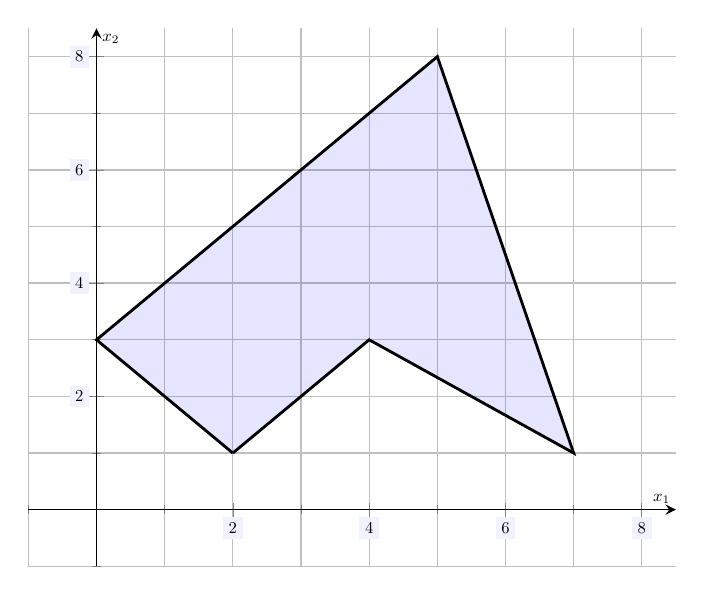
\begin{tikzpicture}[scale=1.2,every node/.style={scale=0.5}]
	\begin{axis}[
	grid=both,
	axis lines=middle,
	ticklabel style={fill=blue!5!white},
	xmin= -1, xmax=8.5,
	ymin= -1, ymax=8.5,
	xtick={0,2,4,6,8},
	ytick={0,2,4,6,8},
	minor tick = {-1,0,1,...,8},
	xlabel=\(x_1\),ylabel=\(x_2\),
	]
	\draw[line width=0.01cm,fill= blue,opacity=0.1] (2,1) -- (0,3) -- (5,8) -- (7,1) -- (4,3) -- (2,1);
	\draw[line width=0.03cm] (2,1) -- (0,3) -- (5,8) -- (7,1) -- (4,3) -- (2,1);
	\end{axis}
	\end{tikzpicture}
	}
	\] \par
Find the maximum and minimum values of $f(x_1, x_2)$ on the region above---if they exist. Be sure to fully justify your answer. \pspace

\sol First, observe that the region is nonempty. For instance, the region contains the point $(4, 4)$ or $(2, 1)$. Second, observe that the region shown is bounded. For instance, it is contained in the rectangle $[0, 8] \times [0, 8]$. Third, observe that the region is closed. Lastly, observe that the function $f(x_1, x_2)= 3x_1 - x_2$ is linear. Therefore, the Fundamental Theorem of Linear Programming states that the function $f(x_1, x_2)$ has a maximum and minimum on the region and that these must occur at a corner point. Therefore, we need only list the corner points and evaluate the function at each of these points. \par
	\begin{table}[!ht]
	\centering
	\begin{tabular}{c|l}
	Corner Point & $f(x_1, x_2)$ \\ \hline
	$(0, 3)$ & $f(0, 3)= 3(0) - 3= 0 - 3= -3$ \\
	$(5, 8)$ & $f(5, 8)= 3(5) - 8= 15 - 8= 7$ \\
	$(7, 1)$ & $f(7, 1)= 3(7) - 1= 21 - 1= 20$ \\
	$(4, 3)$ & $f(4, 3)= 3(4) - 3= 12 - 3= 9$ \\
	$(2, 1)$ & $f(2, 1)= 3(2) - 1= 6 - 1= 5$
	\end{tabular}
	\end{table} \par
Therefore, the minimum value is $-3$ and it occurs at $(x_1, x_2)= (0, 3)$, and the maximum value is $20$ and it occurs at $(x_1, x_2)= (7, 1)$. 
	\[
	\boxed{
	\begin{gathered}
	\min f(x_1, x_2)= -3 \text{ at } (0, 3) \\
	\max f(x_1, x_2)= 20 \text{ at } (7, 1)
	\end{gathered}
	}
	\]



% Question 9
\newpage
\question[10] Find the initial simplex tableau corresponding to the maximization problem shown below. 
	\[
	\begin{gathered}
	\max z= 2.1x_1 + 6.8x_2 - 4.9x_3 \\
	1.1x_1 + 4.8x_2 - 9.0x_3 \leq 17.5 \\
	2.8x_1 + 15.8x_3 \leq 19.4 \\
	7.4x_1 - 5.6x_2 + 6.8x_3 \geq -18.7 \\
	3.1x_1 + 8.8x_2 - 3.1x_3 \geq 14.9 \\
	x_1, x_2, x_3 \geq 0 
	\end{gathered}
	\] 

{\footnotesize
\sol First, observe that this optimization is not in standard form because the third inequality is not `$\leq$' (and the constant term is negative) and the fourth inequality is `$\geq$.' We cannot multiply both sides of the fourth inequality by $-1$ because this would make the constant term negative. So instead, we will introduce a surplus variable for this inequality. Multiplying both sides of the third inequality by $-1$ (and making sure each variable is present in each inequality, in the proper order in the second), we have\dots 
	\[
	\begin{gathered}
	\max z= 2.1x_1 + 6.8x_2 - 4.9x_3 \\
	1.1x_1 + 4.8x_2 - 9.0x_3 \leq 17.5 \\
	2.8x_1 + 0x_2 + 15.8x_3 \leq 19.4 \\
	-7.4x_1 + 5.6x_2 - 6.8x_3 \leq 18.7 \\
	3.1x_1 + 8.8x_2 - 3.1x_3 \geq 14.9 \\
	x_1, x_2, x_3 \geq 0 
	\end{gathered}
	\] 
Now introducing slack variables into the first three inequalities and a surplus variable in the fourth inequality, we have\dots \par
	\begin{table}[!ht]
	\centering
	\begin{tabular}{rrrrrrrrrrrrrrr}
	$1.1x_1$ & $+$ & $4.8x_2$ & $+$ & $-9.0x_3$ & $+$ & $s_1$ &  &  &  &  &  &  & $=$ & $17.5$ \\
	$2.8x_1$ & $+$ & $0x_2$ & $+$ & $15.8x_3$ & $+$ &  &  & $s_2$ &  &  &  &  & $=$ & $19.4$ \\
	$-7.4x_1$ & $+$ & $5.6x_2$ & $+$ & $-6.8x_3$ & $+$ &  &  &  &  & $s_3$ &  &  & $=$ & $18.7$ \\
	$3.1x_1$ & $+$ & $8.8x_2$ & $+$ & $-3.1x_3$ & $+$ &  &  &  &  &  &  & $-s_4$ & $=$ & $14.9$ 
	\end{tabular}
	\end{table} \par
Moving things to the `$z$'-side of the equality in the function, we have $z - 4.6x_1 - 3.1x_2 - 7.9x_3= 0$. Adding this to the table yields\dots \par
	\begin{table}[!ht]
	\centering
	\begin{tabular}{rrrrrrrrrrrrrrrrr}
	&& $1.1x_1$ & $+$ & $4.8x_2$ & $+$ & $-9.0x_3$ & $+$ & $s_1$ &  &  &  &  &  &  & $=$ & $17.5$ \\
	&& $2.8x_1$ & $+$ & $0x_2$ & $+$ & $15.8x_3$ & $+$ &  &  & $s_2$ &  &  &  &  & $=$ & $19.4$ \\
	&& $-7.4x_1$ & $+$ & $5.6x_2$ & $+$ & $-6.8x_3$ & $+$ &  &  &  &  & $s_3$ &  &  & $=$ & $18.7$ \\
	&& $3.1x_1$ & $+$ & $8.8x_2$ & $+$ & $-3.1x_3$ & $+$ &  &  &  &  &  &  & $-s_4$ & $=$ & $14.9$ \\ 
	$z$ & $-$ & $2.1x_1$ & $+$ & $-6.8x_2$ & $+$ & $4.9x_3$ & &  &  &  &  &  &  & & $=$ & $0$ \\ 
	\end{tabular}
	\end{table} \par
This yields the following initial simplex tableau: \par
	\begin{table}[!ht]
	\centering
	\begin{tabular}{rrrrrrr|r}
	$1.1$ & $4.8$ & $-9.0$ & $1$ & $0$ & $0$ & $0$ & $17.5$ \\
	$2.8$ & $0.0$ & $-15.8$ & $0$ & $1$ & $0$ & $0$ & $19.4$ \\
	$-7.4$ & $5.6$ & $-6.8$ & $0$ & $0$ & $1$ & $0$ & $18.7$ \\
	$3.1$ & $8.8$ & $-3.1$ & $0$ & $0$ & $0$ & $-1$ & $14.9$ \\ \hline
	$-2.1$ & $-6.8$ & $4.9$ & $0$ & $0$ & $0$ & $0$ & $0$ \\
	\end{tabular}
	\end{table}
}



% Question 10
\newpage
\question[10] Below is the initial simplex tableau corresponding to some maximization problem. Find the corresponding maximization problem. \par
	\begin{table}[!ht]
	\centering
	\begin{tabular}{rrrrrrrrr}
	$3$ & $-1$ & $2$ & $-1$ & $1$ & $0$ & $0$ & $0$ & $22$ \\
	$1$ & $0$ & $6$ & $9$ & $0$ & $1$ & $0$ & $0$ & $15$ \\
	$-2$ & $1$ & $1$ & $-1$ & $0$ & $0$ & $-1$ & $0$ & $4$ \\
	$1$ & $1$ & $1$& $3$ & $0$ & $0$& $0$ & $1$ & $16$ \\
	$-4$ & $3$ & $-5$ & $1$ & $0$ & $0$ & $0$ & $0$ & $0$
	\end{tabular}
	\end{table} 

{\small
\sol First, we introduce a line to delineate between the variables and the constants and the equalities and the functions. \par
	\begin{table}[!ht]
	\centering
	\begin{tabular}{rrrrrrrr|r}
	{\scriptsize $x_1$} & {\scriptsize $x_2$} & {\scriptsize $x_3$} & {\scriptsize $x_4$} & {\scriptsize $s_1$} & {\scriptsize $s_2$} & {\scriptsize $s_3$} & {\scriptsize $s_4$} & \\
	$3$ & $-1$ & $2$ & $-1$ & $1$ & $0$ & $0$ & $0$ & $22$ \\
	$1$ & $0$ & $6$ & $9$ & $0$ & $1$ & $0$ & $0$ & $15$ \\
	$-2$ & $1$ & $1$ & $-1$ & $0$ & $0$ & $-1$ & $0$ & $4$ \\
	$1$ & $1$ & $1$& $3$ & $0$ & $0$& $0$ & $1$ & $16$ \\ \hline
	$-4$ & $3$ & $-5$ & $1$ & $0$ & $0$ & $0$ & $0$ & $0$
	\end{tabular}
	\end{table} \par
Each row of the tableau `corresponds' to an inequality with the exception of the last row which `corresponds to the function.' But then there were $5 - 1= 4$ inequalities in the original system (ignoring the non-negativity inequality). Because we introduce a slack/surplus variable for each inequality to create an equality, there were four slack/surplus variables. Each column of the tableau `corresponds' to a variable in the system with the exception of the last column which `corresponds to the constants. Therefore, there were $9 - 1= 8$ variables in the system. But because there are four slack/surplus variables, there were $8 - 4= 4$ `original' variables in the system of inequalities. We label the original variables $x_1$, $x_2$, $x_3$, $x_4$, the slack/surplus variables $s_1$, $s_2$, $s_3$, and $s_4$, and the function $z$, which we add to the table above. The last row corresponds to the function. Therefore, we know that $z - 4x_1 + 3x_2 - 5x_3 + x_4 + 0s_1 + 0s_2 + 0s_3 + 0s_4= 0$ so that $z= 4x_1 - 3x_2 - 5x_3 - x_4$. Writing out the equations that correspond to each of the rows (except the last that corresponds to the function), we have\dots
	\[
	\begin{gathered}
	3x_1 - x_2 + 2x_3 - x_4 + s_1= 22 \\
	x_1 + 6x_3 + 9x_4 + s_2= 15 \\
	-2x_1 + x_2 + x_3 - x_4 - s_3= 4 \\
	x_1 + x_2 + x_3 + 3x_4 + s_4= 16
	\end{gathered}
	\]
By assumption, we know that $x_1, x_2, x_3, x_4 \geq 0$. Writing out the inequalities corresponding to the equalities above, we know the original maximization problem was\dots
	\[
	\begin{gathered}
	\max z= 4x_1 - 3x_2 + 5x_3 - x_4 \\
	3x_1 - x_2 + 2x_3 - x_4 \leq 22 \\
	x_1 + 6x_3 + 9x_4 \leq 15 \\
	-2x_1 + x_2 + x_3 - x_4 \geq 4 \\
	x_1 + x_2 + x_3 + 3x_4 \leq 16 \\
	x_1, x_2, x_3, x_4 \geq 0
	\end{gathered}
	\]
}



% Question 11
\newpage
\question[10] Below is the final simplex tableau corresponding to some maximization problem. Find the solution to the original optimization problem. \par
	\begin{table}[!ht]
	\centering
	\begin{tabular}{rrrrrrrrr}
	$0$ & $0$ & $1$ & $0.77$ & $0.13$ & $-0.04$ & $0.04$ & $0$ & $16.21$ \\
	$0$ & $1$ & $0$ & $1.34$ & $0.14$ & $0.05$ & $-0.01$ & $0$ & $22.78$ \\
	$1$ & $0$ & $0$ & $1.78$ & $0.06$ & $0.07$ & $0.08$ & $0$ & $45.55$ \\
	$0$ & $0$ & $0$ & $-7.69$ & $-0.2$ & $-0.79$ & $-0.66$ & $1$ & $24.34$ \\
	$0$ & $0$ & $0$ & $12.58$ & $0.49$ & $0.04$ & $0.55$ & $0$ & $220.34$ 	
	\end{tabular}
	\end{table} 

\sol Each row of the tableau `corresponds' to an inequality with the exception of the last row which `corresponds to the function.' But then there were $5 - 1= 4$ inequalities in the original system (ignoring the non-negativity inequality). Because we introduce a slack/surplus variable for each inequality, there were four slack/surplus variables. Each column of the tableau `corresponds' to a variable in the system with the exception of the last column which `corresponds to the solutions. Therefore, there were $9 - 1= 8$ variables in the system. But because there are four slack/surplus variables, there were $8 - 4= 4$ `original' variables in the system of inequalities. We label the original variables $x_1$, $x_2$, $x_3$, $x_4$, the slack/surplus variables $s_1$, $s_2$, $s_3$, and $s_4$, and the function $z$. Therefore, we need find the maximum value of $z$ along with the values of the variables----namely, the values for $(x_1, x_2, x_3, x_4, x_5, s_1, s_2, s_3, s_4)$. Adding `dividers' to the tableau and `naming' the columns, we have\dots \par
	\begin{table}[!ht]
	\centering
	\begin{tabular}{rrrrrrrr|r}
	{\scriptsize $x_1$} & {\scriptsize $x_2$} & {\scriptsize $x_3$} & {\scriptsize $x_4$} & {\scriptsize $s_1$} & {\scriptsize $s_2$} & {\scriptsize $s_3$} & {\scriptsize $s_4$} & \\
	$0$ & $0$ & $\boxed{1}$ & $0.77$ & $0.13$ & $-0.04$ & $0.04$ & $0$ & $16.21$ \\
	$0$ & $\boxed{1}$ & $0$ & $1.34$ & $0.14$ & $0.05$ & $-0.01$ & $0$ & $22.78$ \\
	$\boxed{1}$ & $0$ & $0$ & $1.78$ & $0.06$ & $0.07$ & $0.08$ & $0$ & $45.55$ \\
	$0$ & $0$ & $0$ & $-7.69$ & $-0.2$ & $-0.79$ & $-0.66$ & $\boxed{1}$ & $24.34$ \\ \hline
	$0$ & $0$ & $0$ & $12.58$ & $0.49$ & $0.04$ & $0.55$ & $0$ & $220.34$ 	
	\end{tabular}
	\end{table} \par
We indicate the pivot positions above. From these pivot positions, we can observe $x_3= 16.21$, $x_2= 22.78$, and $x_1= 45.55$, and $s_4= 24.34$. All remaining variables have value 0. The maximum value is $220.34$. Therefore, the maximum value is $220.34$ and occurs at $(x_1, x_2, x_3, x_4, s_1, s_2, s_3, s_4)= (45.55, 22.78, 16.21, 0, 0, 0, 0, 24.34)$. 
	\[
	\boxed{
	\begin{gathered}
	\max z= 220.34 \text{ at} \\
	(x_1, x_2, x_3, x_4, s_1, s_2, s_3, s_4)= (45.55, 22.78, 16.21, 0, 0, 0, 0, 24.34) \text{, i.e. } \\
	\begin{cases}
	x_1= 45.55 \\
	x_2= 22.78 \\
	x_3= 16.21 \\
	x_4= 0 \\
	s_1= 0 \\
	s_2= 0 \\
	s_3= 0 \\
	s_4= 24.34
	\end{cases}
	\end{gathered}
	}
	\]



% Question 12
\newpage
\question[10] Find the dual problem to the minimization problem shown below. 
	\[
	\begin{gathered}
	\min z= 3x_1 + x_2 + 5x_3 \\
	x_1 + x_2 - x_3 \geq 9 \\
	2x_1 - 5x_2 + x_3 \geq 11 \\
	x_1 - x_3 \geq 6 \\
	x_2 + x_3 \geq 3 \\
	x_1, x_2, x_3 \geq 0 
	\end{gathered}
	\] \pspace

\sol First, observe that the given minimization problem is in standard form; that is, the function is linear, all the inequalities are `$\geq$' a non-negative number, and the variables are non-negative. Because there are variables missing in the inequalities, we introduce them---being sure to keep the $x_1$, $x_2$, $x_3$ `order.' 
	\[
	\begin{gathered}
	x_1 + x_2 - x_3 \geq 9 \\
	2x_1 - 5x_2 + x_3 \geq 11 \\
	x_1 + 0x_2 - x_3 \geq 6 \\
	0x_1 + x_2 + x_3 \geq 3 \\
	\end{gathered}
	\] 
Now we write the `matrix associated' to this minimization; that is, we create a matrix with rows corresponding to the equality version of the inequalities (with the exception of the non-negativity inequality) with the function being the last row. This yields matrix:
	\[
	\begin{pmatrix}
	1 & 1 & -1 & 9 \\
	2 & -5 & 1 & 11 \\
	1 & 0 & -1 & 6 \\
	0 & 1 & 1 & 3 \\
	3 & 1 & 5 & 0 
	\end{pmatrix}
	\]
We now find the transpose of this matrix: 
	\[
	\begin{pmatrix}
	1 & 1 & -1 & 9 \\
	2 & -5 & 1 & 11 \\
	1 & 0 & -1 & 6 \\
	0 & 1 & 1 & 3 \\
	3 & 1 & 5 & 0 
	\end{pmatrix}^T= 
	\begin{pmatrix}
	1 & 2 & 1 & 0 & 3 \\
	1 & -5 & 0 & 1 & 1 \\
	-1 & 1 & -1 & 1 & 5 \\
	9 & 11 & 6 & 3 & 0 
	\end{pmatrix}
	\]
We now find the standard maximization problem corresponding to this matrix:
	\[
	\begin{gathered}
	\max w= 9y_1 + 11y_2 + 6y_3 + 3y_4 \\
	y_1 + 2y_2 + y_3 \leq 3 \\
	y_1 - 5y_2 + y_4 \leq 1 \\
	-y_1 + y_2 - y_3 + y_4 \leq 5 \\
	y_1, y_2, y_3, y_4 \geq 0 
	\end{gathered}
	\] 


\end{questions}
\end{document}